\documentclass[12pt,a4paper]{article}
\usepackage[utf8]{inputenc}
\usepackage{amsmath, amssymb}
\usepackage{graphicx}
\usepackage{geometry}
\usepackage{float}
\usepackage{booktabs}
\usepackage{caption}
\usepackage{circuitikz}
\geometry{a4paper, margin=1in}

\title{\textbf{09. Amplitude modulation}}
\author{Yamulapalli Nandu Navadeep \\ Roll Number: IMS24267}
\date{Date of Experiment: 10/08/2026 \\ Date of Submission: 30/08/2026}

\begin{document}

\maketitle

\section{Aim of the Experiment}
\begin{enumerate}
    \item To design and set up an amplitude modulator using transistor
    \item To measure the modulation index for different amplitudes of the audio signal.
\end{enumerate}

\section{Theory}
Amplitude modulation (AM) is a process where the amplitude of a high-frequency carrier wave is changed according to the amplitude of a low-frequency signal (like audio). We cannot transmit audio waves directly over long distances because they would need extremely large antennas. High-frequency radio waves, however, can travel long distances with smaller antennas. Therefore, we combine the low-frequency audio signal with a high-frequency carrier wave for transmission.

The \textit{modulation index} ($m_a$) measures how much the carrier wave's amplitude changes. It is calculated by measuring the maximum ($V_{max}$) and minimum ($V_{min}$) voltages of the modulated signal's envelope.

The value of $m_a$ tells us how strong the modulation is. Usually, $m_a$ is between 0 and 1. When $m_a = 1$, it is called 100\% modulation or critical modulation, which gives the strongest signal without distortion. If $m_a > 1$, it is called \textit{over modulation}. Over modulation causes the signal to distort, so it should be avoided. When $m_a < 1$, it is called \textit{under modulation}.

\begin{itemize}
    \item $|m_a| < 1$: Under modulation
    \item $|m_a| = 1$: Critical modulation
    \item $|m_a| > 1$: Over modulation
\end{itemize}

\section{Procedure}
\begin{enumerate}
    \item Connect the circuit as per the circuit diagram.
    \item Apply a high-frequency carrier signal to the base of the transistor and a low-frequency modulating signal to the emitter.
    \item Observe the output on the oscilloscope.
    \item Vary the amplitude of the modulating signal to obtain under modulation, critical modulation, and over modulation.
    \item Measure the $V_{max}$ and $V_{min}$ from the envelope of the output signal for each case.
    \item Calculate the modulation index $m_a$ for each case.
\end{enumerate}

\section{Circuit Diagram}
\begin{figure}[H]
\centering
\begin{circuitikz}[scale=0.8, transform shape]
    \draw (0,0) node[npn] (Q1) {BC107};
    
    % Biasing network
    \draw (Q1.B) to[short] (-2,0) coordinate (B);
    \draw (B) to[R, l=$22\text{ k}\Omega$] ++(0,3.8) coordinate (VCC1);
    \draw (B) to[R, l=$6.8\text{ k}\Omega$] ++(0,-3) coordinate (GND_NODE) node[ground]{};
    \draw (B) to[R, l=$1\text{ k}\Omega$] ++(-2,0) to[sV, l=Carrier] ++(0,-2) node[ground]{};

    % Emitter
    \draw (Q1.E) to[R, l=$10\text{ k}\Omega$] ++(0,-2) coordinate (E1);
    \draw (E1) to[sV, l=Signal] (E1 |- GND_NODE) to[short] (GND_NODE);

    % Collector and LC tank
    \draw (Q1.C) to[short] ++(0,1) coordinate (C1);
    \draw (C1) to[short] ++(-1.25,0) to[L, l=$100\text{ mH}$] ++(0,2) coordinate (TC1);
    \draw (C1) to[short] ++(1.25,0) to[C, l=$0.01\text{ }\mu\text{F}$] ++(0,2) coordinate (TC2);
    \draw (TC1) to[short] (TC2);
    \draw (TC1) ++(0,0) coordinate (VCC2);
    \draw (VCC1) to[short] (VCC2);
    \draw (VCC2) to[short] ++(1,0) node[vcc] {$V_{CC} = 7\text{ V}$};
    
    % Output
    \draw (Q1.C) to[short, *-o] ++(3.5,0) node[right] {$V_{out}$};
\end{circuitikz}
\caption{Circuit diagram of Amplitude Modulator}
\end{figure}

\section{Tabular Column}
\textbf{Given Parameters:}
\begin{itemize}
    \item Carrier Frequency ($f_c$): $3.9 \text{ kHz}$
    \item Modulating Signal Frequency ($f_m$): $0.18 \text{ kHz}$
\end{itemize}

\begin{table}[H]
\centering
\begin{tabular}{|c|c|c|c|c|}
\hline
\textbf{Case} & \textbf{Condition} & \textbf{$V_{max}$ (mV)} & \textbf{$V_{min}$ (mV)} & \textbf{Modulation Index ($m_a$)} \\
\hline
Under modulation & $c > s$ & 400 & 120 & 0.54 \\
Critical modulation & $c = s$ & 520 & 20 & 0.93 \\
Over modulation & $c < s$ & 712 & 192 & 3.7 \\
\hline
\end{tabular}
\caption{Observations for Modulation Index}
\end{table}
\noindent*(Note: $c$ is the carrier signal amplitude and $s$ is the modulating signal amplitude)*

\section{Calculations}
The theoretical resonant frequency of the LC tank circuit is given by:
$$f_r = \frac{1}{2\pi\sqrt{LC}} = \frac{1}{2\pi\sqrt{100 \times 10^{-3} \times 0.01 \times 10^{-6}}} \approx 5.03 \text{ kHz}$$
This is in the same range as the applied carrier frequency of 3.9 kHz, allowing the tank to act as a band-pass filter for the carrier and its sidebands.

\subsection{Under Modulation ($c > s$)}
For under modulation, the envelope does not reach zero. The modulation index is calculated as:
$$m_a = \frac{V_{max} - V_{min}}{V_{max} + V_{min}}$$
$$m_a = \frac{400 - 120}{400 + 120} = \frac{280}{520} \approx 0.54$$

\subsection{Critical Modulation ($c = s$)}
$$m_a = \frac{V_{max} - V_{min}}{V_{max} + V_{min}}$$
$$m_a = \frac{520 - 20}{520 + 20} = \frac{500}{540} \approx 0.93$$

\subsection{Over Modulation ($c < s$)}
For over modulation, the envelope crosses the zero axis and gets distorted. The formula for the modulation index in this case is:
$$m_a = \frac{V_{max}}{V_{min}}$$
$$m_a = \frac{712}{192} \approx 3.7$$

\section{Results}
An amplitude modulator was successfully set up using a BC107 transistor. The modulation index was calculated for different amplitudes of the audio signal. The values were found to be:
\begin{itemize}
    \item Under modulation: $m_a = 0.54$
    \item Critical modulation: $m_a = 0.93$
    \item Over modulation: $m_a = 3.7$
\end{itemize}

Theoretical waveforms of under, critical and over modulation were observed on the DSO as per the theory.


\section{Discussion}
In this experiment, we successfully created an amplitude modulated signal using a simple transistor circuit. We applied a high-frequency carrier signal (3.9 kHz) to the base of the transistor and a low-frequency audio signal (0.18 kHz) to the emitter.

The LC tank circuit at the collector worked as a band-pass filter. Its theoretical resonant frequency was around 5.03 kHz. This allowed the carrier frequency and its sidebands to pass through to the output while blocking unwanted low frequencies.

By changing the amplitude of the audio signal, we observed three different types of modulation. In \textbf{under modulation} ($m_a = 0.54$), the output envelope followed the audio signal without hitting zero. When we increased the audio signal's amplitude to match the carrier, we reached \textbf{critical modulation} ($m_a = 0.93 \approx 1$), where the envelope's minimum points almost touched zero. When we increased the audio signal's amplitude even more, we got \textbf{over modulation} ($m_a = 3.7$). This caused the envelope to flip and distort, which is bad for real-world communication systems.

\section{References}
\begin{enumerate}
    \item Lab Manual for Advanced Physics Lab II, IISER TVM.
    \item Boylestad, R. L., \& Nashelsky, L., \textit{Electronic Devices and Circuit Theory}, Pearson.
\end{enumerate}

\section{Lab Notes (Observations)}
The following handwritten notes and observations were recorded during the laboratory session.

\begin{figure}[H]
    \centering
    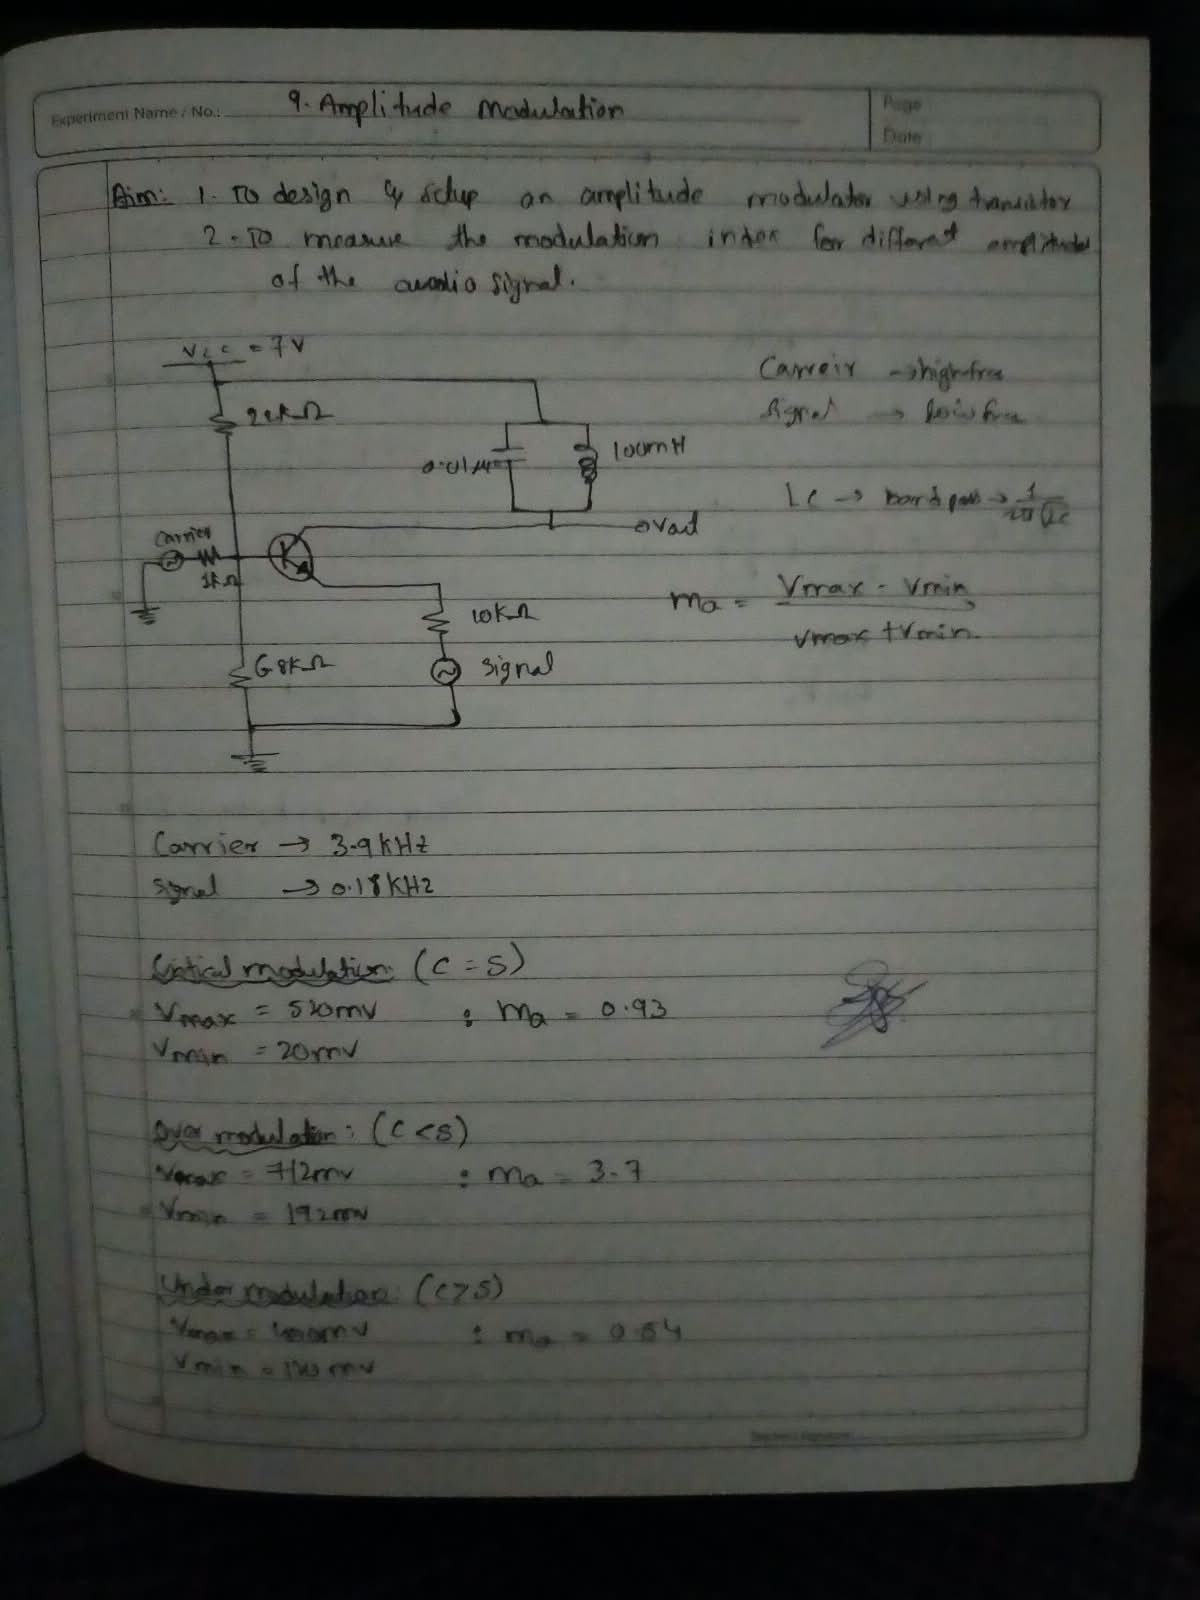
\includegraphics[width=0.85\textwidth]{observation.jpeg}
    \caption{Lab Notes for Amplitude Modulation}
\end{figure}

\end{document}
